%%%%%%%%%%%%%%%%%%%%%%%%%%%%%%%%%%%%%%%%%%%%%%%%%%%%%%%%%%%%%%%%%%%%%%%%%%%%%%%%%%%%%%%%%%%%%%%%%%%%%%%%%%%%%%%%%%%%%%%%%%%%%%%%%%%%%%%%
% This is just a template to use when submitting manuscripts to Frontiers, it is not mandatory to use frontiers.cls nor frontiers.tex  %
%%%%%%%%%%%%%%%%%%%%%%%%%%%%%%%%%%%%%%%%%%%%%%%%%%%%%%%%%%%%%%%%%%%%%%%%%%%%%%%%%%%%%%%%%%%%%%%%%%%%%%%%%%%%%%%%%%%%%%%%%%%%%%%%%%%%%%%%

\documentclass{frontiersSCNS} % for Science articles
%\documentclass{frontiersMED} % for Medicine articles

\usepackage{url}

%\usepackage{lineno}
\usepackage{todonotes}


% Absolute numerotation for figures
\usepackage{caption}
\usepackage{subcaption}
\captionsetup{figurewithin=none}  
\captionsetup{tablewithin=none}
%\usepackage[tight]{subfigure}
\def\subfigbottomskip{0pt}

\usepackage{listings}
\lstset{language=python,
	basicstyle=\ttfamily,
	extendedchars=true,
	xleftmargin = 0pt,
	rulecolor=\color{black!50},
        aboveskip = 0.5ex,
        belowskip = 0.6ex,
	escapebegin={\color{green!50!black}},
        %keywordstyle=\sffamily\bfseries\color{grey},
	%identifierstyle=\sffamily,
	commentstyle=\slshape\color{green!50!black},
	stringstyle=\rmfamily\color{blue},
	showstringspaces=false,
	tabsize=2,
	breaklines=true,
	%classoffset=1,
        morekeywords={{,},=,:},
	%classoffset=0,
        frame=single,xleftmargin=\fboxsep,xrightmargin=-\fboxsep
    }
	

%\makeatletter
% Space between floats
%\setlength\floatsep    {4\p@}
% Space between floats and text
%\setlength\textfloatsep{4\p@}
% Space above and below an inline figure
%\setlength\intextsep   {4\p@}
%\makeatother


\newcommand{\alex}[1]{\todo[inline, color=green!40]{#1}}
\newcommand{\fabian}[1]{\todo[inline, color=blue!40]{#1}}



%\linenumbers


\copyrightyear{}
\pubyear{}
%\onecolumn
%%% write here for which journal %%%
\def\journal{Neurosciences}
\def\DOI{}
\def\articleType{}
\def\citing{\color{darkgray}\cite}
\def\keyFont{\fontsize{6}{11}\helveticabold }
\def\firstAuthorLast{Alexandre Abraham {et~al}} %use et al only if is more than 1 author

% XXX Review the order of authors

\def\Authors{
    Alexandre Abraham\,$^{1,2,*}$,
    Fabian Pedregosa\,$^{1,2}$,
    Michael Eickenberg\,$^{1,2}$,
    Philippe Gervais\,$^{1,2}$,
    Andreas Muller,
    Jean Kossaifi,
    Alexandre Gramfort\,$^{1,2,3}$,
    Bertrand Thirion\,$^{1,2}$
    and Ga\"el Varoquaux\,$^{1,2}$}
% Affiliations should be keyed to the author's name with superscript numbers and be listed as follows: Laboratory, Institute, Department, Organization, City, State abbreviation (USA, Canada, Australia), and Country (without detailed address information such as city zip codes or street names).
% If one of the authors has a change of address, list the new address below the correspondence details using a superscript symbol and use the same symbol to indicate the author in the author list.
\def\Address{
    $^{1}$Parietal Team, INRIA Saclay-\^{I}le-de-France, Saclay, France\\
    $^{2}$Neurospin, I\textsuperscript{2}BM, DSV, CEA, 91191 Gif-Sur-Yvette, France\\
    $^{3}$Institut Mines-Telecom, Telecom ParisTech, CNRS LTCI, 75014 Paris, France}

% The Corresponding Author should be marked with an asterisk
% Provide the exact contact address (this time including street name and city zip code) and email of the corresponding author
\def\corrAuthor{Alexandre Abraham}
\def\corrAddress{Parietal Team, INRIA Saclay-\^{I}le-de-France, Saclay, France}
\def\corrEmail{alexandre.abraham@inria.fr}

% \color{FrontiersBlue} Is the blue color, used in the Journal name, in the title, and the names of the sections

% Bunch of code for 3D cubes

% Example of table from template

% \begin{table}[!t]
% \processtable{Resolution Requirements for the figures\label{Tab:01}}
% {\begin{tabular}{lllll}\toprule
% Image Type & Description & Format & Color Mode & Resolution\\\midrule
% Line Art & An image composed of lines and text,  & TIFF, EPS, JPEG & RGB, Bitmap & 900 - 1200 dpi\\
%            & which does not contain tonal or shaded areas.& & &\\
%            Halftone & A continuous tone photograph, which contains no text. & TIFF, EPS, JPEG & RGB, Grayscale & 300 dpi\\
% Combination & Image contains halftone + text or line art elements. & TIFF, EPS, JPEG & RGB,Grayscale & 600 - 900 dpi\\\botrule
% \end{tabular}}{This is a footnote}
% \end{table}


% Figures

% \textbf{Figure 1.}{ Enter the caption for your figure here.  Repeat as  necessary for each of your figures.}\label{fig:01}
% Don't add the figures in the LaTeX files, please upload them when submitting the article. Frontiers will add the figures at the end of the provisional pdf.


%%%%%%%%%%%%%%%%%%%%%%%%%%%%%%%%%%%%%%%%%%%%%%%%%%%%%%%%%%%%%%%%%%%%%%%%%%%%%%%
%%%%%%%%%%%%%%%%%%%%%%%%%%%%%%%%%%%%%%%%%%%%%%%%%%%%%%%%%%%%%%%%%%%%%%%%%%%%%%%
%%%%                                                                       %%%%
%%%%                          Naming convention                            %%%%
%%%%                                                                       %%%%
%%%%%%%%%%%%%%%%%%%%%%%%%%%%%%%%%%%%%%%%%%%%%%%%%%%%%%%%%%%%%%%%%%%%%%%%%%%%%%%
%%%%%%%%%%%%%%%%%%%%%%%%%%%%%%%%%%%%%%%%%%%%%%%%%%%%%%%%%%%%%%%%%%%%%%%%%%%%%%%

% Nifti world
% -----------
% - func_filename: name of a dataset file
% - func_img: name of a (loaded) nifti file
% - func_data, func_affine: data and affine of functional data

% Scikit-learn world
% ------------------
% - Xs: list of unmasked func_data (scikit-learn world)
% - X: unmasked func_data reduced to 2 dimensions (scikit-learn world)
% - y: labels

\begin{document}
\onecolumn
\firstpage{1}

\title[Machine Learning for Neuroimaging with Scikit-Learn]{Machine Learning for Neuroimaging with Scikit-Learn}
\author[\firstAuthorLast ]{\Authors}
\address{}
\correspondance{}
\editor{}
\topic{Research Topic}

\maketitle
\begin{abstract}

\section{}
Statistical machine learning methods are increasingly used for
neuroimaging data analysis. Their main virtue for this type of application
is their ability to model high-dimensional datasets, e.g.\ multivariate
analysis of activation images, or capturing inter-subject variability.
Supervised learning is typically used in \emph{decoding} or
\emph{encoding} settings to relate
brain images to behavioral or clinical observations, while
unsupervised learning is typically used to uncover hidden structure in
sets of images (e.g.\ resting state functional MRI) or to find
sub-populations in large cohorts of subjects. By considering
different functional neuroimaging applications, we illustrate how scikit-learn,
a Python machine learning library, can be used to perform some key
analysis steps. Scikit-learn contains a large set of statistical
learning algorithms, both supervised and unsupervised, that can be applied
to neuroimaging data. Other Python libraries provide the tools for
loading and preparing neuroimaging data for scikit-learn, and visualizing
the results.

% XXX: here the tone of the article should be: scikit-learn for methods
% development, ie we target the methods researchers for Neuroimaging. We
% should make this explicit in the intro and conclusion

\tiny
% XXX Fix keywords
%All article types: you may provide up to 8 keywords; at least 5 are mandatory.
\section{Keywords:} machine learning, statistical learning, neuroimaging,
scikit-learn, Python
\end{abstract}


\section{Introduction}

Statistical machine learning is gaining interest in
neuroimaging data analysis. It is used by neuroscientists,
who use machine learning methods as black boxes, and computer scientists,
who acquire neuroscientific knowledge on the job. This paper aims to fill 
the gap between machine learning and neuroimaging by demonstrating how a 
general-purpose machine-learning toolbox can be used to produce scripts 
for neuroimaging analysis with state-of-the-art methods
that are fully understood by both worlds.

With its mature scientific stack, Python is a growing contender in the
landscape of neuroimaging data analysis with tools such as Nipy
\citep{millman2007analysis} or Nipype \citep{gorgolewski2011} and some
frameworks for multi-variate pattern analysis already exists
\citep{hanke2009pymvpa}. 

In this paper, we show how scikit-learn, a Python machine learning
library \citep{pedregosa2011}, can be used on neuroimaging data.
Statistical learning can be a useful tool for scientific investigation in
imaging neurosciences in many ways. We discuss a few applications to
resolve common neuroimaging needs, which methods can be used, what they
imply and how to achieve the desired results. We discuss not only
prediction scores, but also the interpretability of the results, which
leads us to open up the black box methods. The paper is organized as
follows. After introducing the \emph{scikit-learn} toolbox, we show 
how the data must be prepared to apply
\emph{scikit-learn}. Then we describe the application of \emph{supervised
learning} techniques, to learn the links between brain images and
stimuli. Finally we demonstrate how \emph{unsupervised learning}
techniques can extract useful structure from the images.

% Maybe we should stress that this paper is meant to be didactic, and
% thus only presents simple examples

\subsection{Scientific Python and neuroimaging ecosystem}

Thanks to its scientific libraries, Python is able to compete with languages
originally made for scientific computation like Matlab or R. The main libraries
are:
\begin{itemize}
    \item{\bf Scipy and Numpy} packages are the basis of scientific computing in Python.
        NumPy provides the \verb!ndarray! data type, an efficient $n$-dimensional data
        representation for array-based numerical computating, a la Matlab
        \citep{vanderwalt2011}.
        SciPy provides higher level mathematical functions that operate on ndarrays for
        a variety of domains including linear algebra, optimization and signal
        processing. Together, NumPy and SciPy provide a robust scientific environment
        for numerical computing and they are the elementary bricks we use in all our
        algorithms.

    \item{\bf Matplotlib} is a plotting library tightly integrated into the
        the scientific Python stack \citep{hunter2007}. It offers publication-quality figures in
        a variety of formats and can display plots or images in a
        graphical user interface. All figures in this paper have been generated using
        it.

    \item{\bf Nibabel} loads or saves data in neuroimaging file formats.
	We use it at the beginning of all our scripts.
\end{itemize}

\section{Scikit-learn}
\label{scikitlearn}

{\em Scikit-learn} \citep{pedregosa2011} is an open source machine
learning library for the Python programming language. The ambition of the
project is to provide efficient and well-established machine learning tools within
a programming environment that is accessible to non-machine learning experts
and reusable in various scientific areas.

\subsection{Concepts}

In {\em scikit-learn}, all objects and algorithms accept data represented
in a generic domain-independent 2-dimensional array, samples $\times$
features. Scikit-learn objects share a uniform set of methods that
depends on their purpose: \textit{estimators} can build and fit models,
\textit{predictors} can make predictions and \textit{transformers}
converting data from one representation to another.

\begin{itemize}
\item {\bf Estimator}. The \textit{estimator} interface, the core of the
    library, exposes a \texttt{fit} method for learning a model from training data.
    All supervised
    and unsupervised learning algorithms (e.g., for classification, regression or
    clustering) are offered as objects implementing this interface. Machine
    learning tasks such as feature extraction, feature selection or dimensionality
    reduction are also provided as estimators.

\item {\bf Predictor}. The \textit{predictor} interface extends the notion of an estimator
    by adding a \texttt{predict}
    method that takes an array \texttt{X\_test} and produces
    predictions for \texttt{X\_test}, based on the learned parameters of the
    estimator (we call the input to \texttt{predict} ``\texttt{X\_test}'' in order
    to emphasize that \texttt{predict} generalizes to new data). In the case of
    supervised learning estimators, this method typically returns the predicted
    labels or values computed by the model.

\item {\bf Transformer}. As it is common to modify or filter data before feeding it to a learning
    algorithm, some estimators in the library implement a \textit{transformer}
    interface which defines a \texttt{transform} method. Preprocessing, feature selection and
    dimensionality reduction
    algorithms are all provided as transformers within the library. If the transformation
    can be inverted, a method called \verb!inverse_transform! also exists.

\end{itemize}

\subsection{Cross validation and model selection}

% XXX: describe cross-validation

The problem of model selection is to find the hyper-parameters or the
model that works best on the data, according for a specific task, most
often prediction on unseen data.
%
In {\em scikit-learn}, model selection can be done with the
\texttt{GridSearchCV} estimator. It takes as input an estimator, whose
hyper-parameters must be optimized, and a set of hyperparameter settings
to search through. 

\section{Data preparation: from MR volumes to a data matrix}

Before applying statistical learning to neuroimaging data, standard
preprocessing must be applied. For fMRI, these namely entail motion
correction, slice timing, coregistration and normalization on a common
template like MNI if necessary. Reference softwares for this task are
SPM\footnote{http://www.fil.ion.ucl.ac.uk/spm}~\citep{friston2007} and
FSL\footnote{http://fsl.fmrib.ox.ac.uk}~\citep{smith2004}. A Python
interface to these tools is available in nipype Python library
\citep{gorgolewski2011}. Below we discuss shaping preprocessed data into
a format that can be fed to scikit-learn. For the machine learning
settings, we need a data matrix, that we will denote $X$, and optionally a
target variable to predict, $y$.

\subsection{Spatial resampling}
\label{resampling}

Neuroimaging data often come as Nifti files, 4-dimensional data (3D scans
composed of voxels and their associated time series) along with a
transformation matrix (called affine) used to compute voxel locations
from data indices to world coordinates. Such matrix can express data
anisotropy, when the distance between two voxels is not the same
depending on the direction. This information is used by algorithms
relying on the spatial structure of the data, for instance the
Searchlight. SciPy provides routines taking affine into account in its
ndimage module, for instance \texttt{scipy.ndimage.affine\_transform}.
% XXX: here, maybe mention nilearn

Resampling consists in changing the spatial resolution of the data. This is
an interpolation and alters the data, that is why it should be used carefully.
Oversampling (increasing data resolution) leads to higher memory consumption
and computation resources with no gain in information.
Downsampling is commonly used to reduce the size of data to process.
Typical sizes are 2mm or 3mm resolutions, but scan spatial resolution is
increasing with progress in MR physics.
Data scaling factor for each direction can be modified in the affine matrix.

\subsection{Signal cleaning}

Due to its acquisition process and poor resolution, neuroimaging data often has a low
signal-to-noise ratio. It contains trends and artifacts that must be removed
to ensure maximum machine learning algorithms efficiency. Signal cleaning
includes:
\begin{itemize}
    \item{\bf Detrending} removes a linear trend over the time series of each
        voxel. This is a useful step when studying fMRI data, as the voxel
        intensity itself has no meaning and we want to study its variation and
        correlation with other voxels. Detrending can be done thanks to SciPy
        (\texttt{scipy.signal.detrend}).
    \item{\bf Normalization} consists in setting the timeseries variance to 1.
        This harmonization is necessary as some machine learning algorithms are
        sensible to different value ranges.
    \item{\bf Confounds removal} consists in regressing out confounding factors.
        Typical neuroimaging confounds are head movements. These spurious
        variables induce spurious correlation between all brain voxels.
        Some datasets provide estimated confounds (usually in csv files) but
        they can also be estimated from the data \citep{behzadi2007}.
    \item{\bf Frequency filtering} consists in removing high or low
        frequency signals. Low-frequency signals in fMRI data are caused by
        physiological mechanisms or scanner drifts.
\end{itemize}

\subsection{From 4-dimensional images to 2-dimensional array: masking}

Neuroimaging data are represented in 4 dimensions: 3 spatial dimensions, and 
one dimension for the time.
Scikit-learn algorithms, on the other hand, only accept 2-dimensional
samples $\times$ features matrices (see \ref{scikitlearn}).
Depending on the settings, voxels and time series can be
considered as features
or samples. For example, in spatial independent component analysis (ICA),
voxels are samples.


Reducing the data dimension from images to feature vectors implies losing its
spatial structure. However, that not all voxels in fMRI data holds 
relevant information: outer-brain voxels are of no
use and, worse, they may bring spurious noise and scanner artifacts.
Thus, we keep only voxels in a brain mask. Such masks
are often given along with datasets or can be computed thanks to softwares like
FSL or SPM.

\begin{figure}[hbtp]
    \begin{center}
        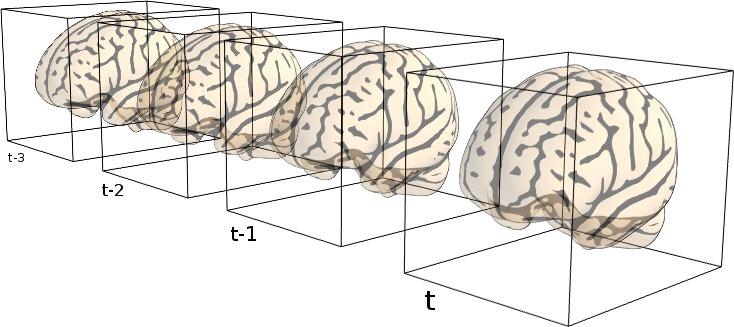
\includegraphics[width=.5\linewidth]{img/niimgs.jpg}
    \end{center}
    \caption{Conversion of brain scans into 2-dimensional data}
    \label{fig:niimg}
\end{figure}

Applying the mask is made easy by NumPy fancy indexing (importantly, the
type of the mask array must be boolean for the following to work).
2-dimensional masked data will be refered as \texttt{X} to follow
scikit-learn conventions:
\begin{lstlisting}
# Ensure that the mask is boolean
mask = mask.astype(np.bool)
# Apply the mask, X = timeseries * voxels
X = func_data[mask].T

# Unmask data
unmasked_data = np.zeros(mask.shape, dtype=X.dtype)
unmasked_data[mask] = X
\end{lstlisting}


% This part has been removed because automatic masking is overly complicated and
% does not brinautomatic masking is overly complicated and does not bring much
% to the paper.

% \subsubsection{Automatically computing a mask}

% The simplest strategy to compute a mask is a binarization by a selected threshold.
% Due to the nature of the neuroimaging data, there exists some strategy to choose
% this threshold in order to obtain a decent segmentation.

% \alex{There is a reference for the method used in Nisl. We should put it there
% and in the code. Add a figure with an histogram to illustrate.}

% Multi subject computation is simply done by intersecting subjects maps
% relatively to a chosen threshold.

%\subsubsection{Label shifting}
%
%Functional MRI acquisition is not immediate: BOLD response peak occurs between 3
%and 5 seconds after the stimulus. We take this time shift into account by
%shifting values of the label array by an offset of 2 time repetition (about 5
%seconds).

% Functional MRI measures brain activity by using the Blood-Oxygen-Level-Dependent
% contrast (BOLD). In fact, like muscles, brain regions consume more oxygen and
% nutriments when stimulated. So when a part of the brain starts working,
% physiological mechanisms induce an oxygen-rich blood flood toward this
% particular region: this is called haemodynamic response.

% However, this reaction takes time, usually around 3-4 seconds. This is the
% duration between the event and the reaction observed in the brain. To be able to
% match these two events, we will sometimes have to shift our data. The number of
% scans that must be shifted depends on the TR (repetition time) of the data.
% Usually, we remove the first two scans of the data and the two last values of the
% labels (to keep an homogeneous length).

%\begin{lstlisting}
%X = X[2:]
%y = y[:-2]
%\end{lstlisting}

\section{Decoding object representation in the brain}

In the context of machine learning in neuroimaging, \textit{decoding} refers to learning a model
which predicts behavioral or phenotypic data given brain activity. 
The reverse procedure is
called \textit{encoding} \citep{naselaris2011} and is introduced in the next 
section.

Here we illustrate decoding with a simpler version of the experiment presented in
\cite{haxby2001}. In the original work, visual stimuli representing 8 different categories
are presented to 6 subjects during 12 sessions. The goal is to 
predict the category of the stimulus presented to subject given his
brain activity. For the sake of simplicity, we will restrict our code 
to one subject for the
particular task of discriminating face against house images.

As there is a \emph{target} variable to predict, $y$, this is a supervised
learning problem. Here $y$ represents a small number of object categories,
\emph{classes} in machine-learning terms. In these settings, the learning
task is known as a \emph{classification} problem, as opposed to a
\emph{regression} problem, for a variable $y$ taking continuous values,
such as age.
Among all methods proposed in the scikit-learn, we will
combine the use of univariate feature selection and Support Vector
Machines (SVM) for this problem. Indeed, this is a common and efficient
setup used in NeuroImaging.

\subsection{Feature selection: ANOVA F-Test}

After applying a brain mask, the data consist of 40\,000 features for 
only 1\,400 samples. Machine learning with much more features than samples
is challenging, due to the so-called \emph{curse of dimensionality}.
A popular strategy is to reducing the number of features (ie voxels) by
selecting the most relevant ones. Based on prior neuroscientific
knowledge, we could restrain the mask to occipital area where the visual
cortex is located. A simple statistical approach relies on screening
features based on a univariate statistical test.

Scikit-learn offers a panel of strategies to select features. In supervised
learning, the most popular feature selection method is the
ANalysis Of VAriance (ANOVA) F-Test. 
The null hypothesis of this test is that the feature takes the same value
for all classes of $y$ to predicted.

After ranking the features, \verb!sklearn.feature_selection! proposes a panel
of feature selection strategies. One can choose to take a percentile of the features
(\verb!SelectPercentile!), or a fixed number of features (\verb!SelectKBest!).
All these objects are implemented as transformers (see
\ref{scikitlearn}) and are easily invertible (see code below).
In this use case, \verb!f_classif! function (ANOVA F-Test) along with selection
of a fixed number of features will be used.

\subsection{Classification: SVM}

A linear Support Vector Classifier (SVC) finds the linear hyperplane that
separates samples belonging to different classes while maximizing the
distance to the samples (called margin). Classifying a new sample boils
down to determining on which side of the hyperplane it lies. A SVC bases
its decision upon a subset of training data called support vectors. As
the linear SVC is a linear classifier, it's decision is based on a set of
weights that form a brain map (see figure~\ref{fig:haxby}).

\begin{lstlisting}
feature_selection = SelectKBest(f_classif, k=500)
clf = SVC(kernel='linear')
X_red = feature_selection.fit_transform(X)
clf.fit(X_red, y)
\end{lstlisting}

% \subsubsection{Pipeline}

% The workflow described above (feature selection + estimator) is a standard one.
% In fact, in most cases, it will consist in atomic steps
% \textit{linked} together (the output of a step is the input of the next one).
% For this purpose, scikit-learn offers a pipeline object that allows such
% linking. A pipeline is simply a list of scikit-learn objects through which the
% input data will be conveyed. The function to call for each object (transform,
% fit...) depends on its type.
% This allow developpers to create new estimators based on existing ones.

% \begin{lstlisting}
% anova_svc = Pipeline([('anova', feature_selection), ('svc', clf)])
% anova_svc.fit(X)
% sv = anova_svc.inverse_tranform(clf.support_vectors_)
% \end{lstlisting}

\subsection{Searchlight}
\label{searchlight}

Searchlight \citep{kriegeskorte2006} is a popular algorithm in the
neuroimaging community. It runs a predictive model on a spatial
neighbourhood of each voxel and tests the out-of-sample prediction
performance as proxy measure of the link between the local brain activity
and the target behavioral variable. In practice, it entails performing
cross-validation of the model, most often an SVM, on voxels contained in
balls centered on each voxel of interest. The procedure amounts to
solving a large number of SVMs and can be computationally expensive.
An efficient implementation of this algorithm is beyond the scope of this
paper and it is not detailed here. However, the code, along with this example,
are available in nilearn\footnote{http://nilearn.github.io}.

\subsection{Results}

The results of this experience are shown in figure~\ref{fig:haxby}.
On all figures, green, resp.\ blue,
lines surround features corresponding to face, resp.\ house, recognition
exhibited in the reference paper.
The F-score (left) is the basic
classifier used in ANOVA to select the features. The middle picture shows the
first support vector obtained with SVC after feature selection. The picture on
the right shows the Searchlight map.

First, we observe that highlighted voxels located in the blue areas are
highlighted by all methods. The Searchlight is more blurry than the other
methods because it iterates over a ball around the voxels.

These results are also neuroscientifically plausible as the activation occurs in the
high level regions of the visual cortex which is known to contain semantic
information about vision. While Searchlight only gives a score to each voxel,
the SVC can be used afterward to classify unseen brain scans.

% XXX has 'SVC' been defined?

\begin{lstlisting}
### Look at the discriminating weights
coef = clf.coef_
# reverse feature selection
coef = feature_selection.inverse_transform(coef)
\end{lstlisting}

\begin{figure}[hbtp]
  \begin{center}
  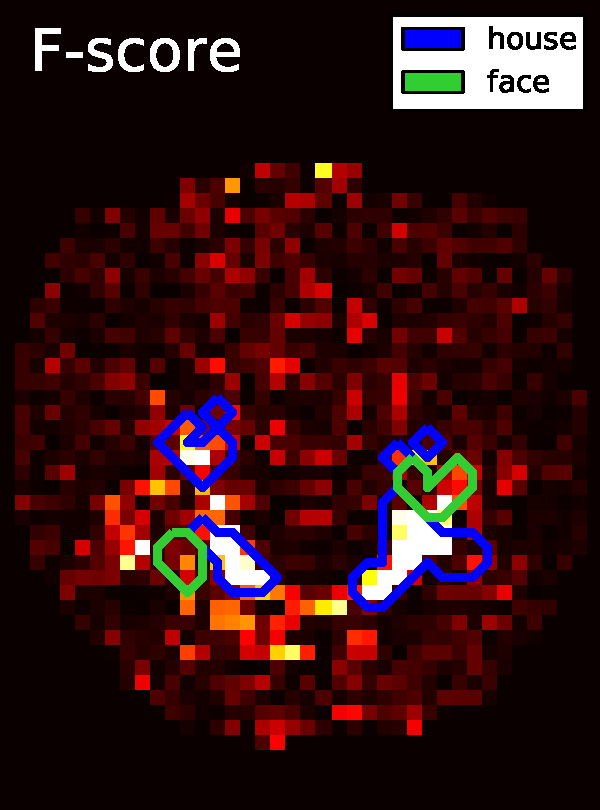
\includegraphics[width=.3\linewidth]{img/haxby/haxby_fscore}
  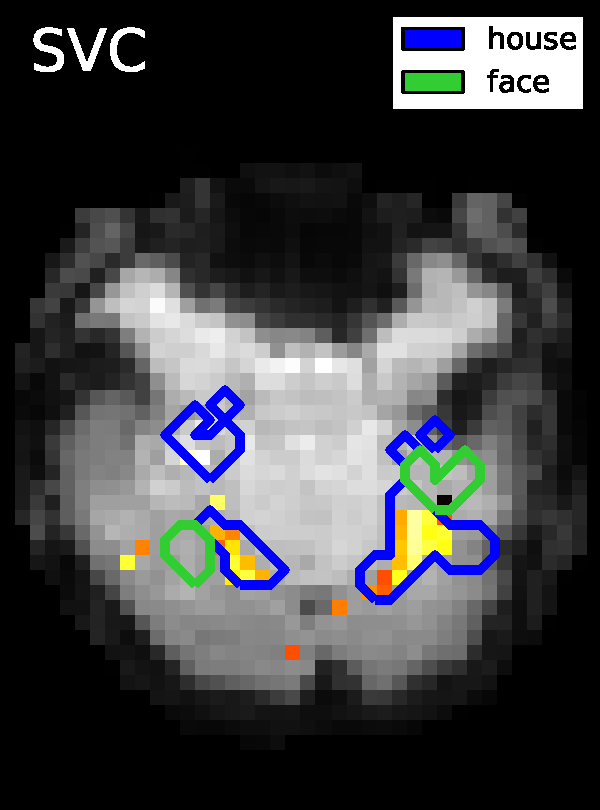
\includegraphics[width=.3\linewidth]{img/haxby/haxby_svm}
  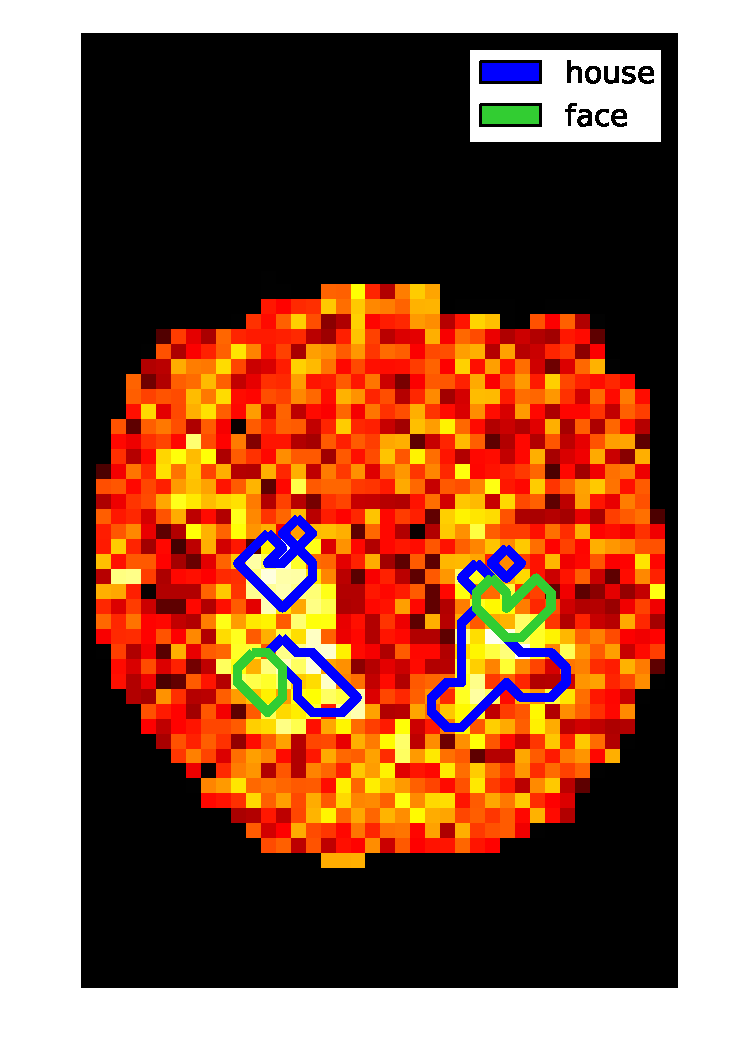
\includegraphics[width=.3\linewidth]{img/haxby/haxby_searchlight}
  \end{center}
\caption{Maps derived by different methods for face versus house
recognition in the Haxby experiment -- \emph{left}: standard analysis;
SVM weights after screening voxels with an anova; \emph{right}:
Searchlight map. The masks derived from standard analysis in the original
paper \citep{haxby2001} are displayed blue and in green.}
\label{fig:haxby}
\end{figure}

% This is too technical
%
% \subsubsection{Implementation}
% 
% Even if this algorithm seems complicated, it can be easily implemented thanks to
% some basic bricks provided by the scikit-learn. They key elements here are
% \textit{i)} the neighbourhood (\texttt{sklearn.neighbors.NearestNeighbors}),
% \textit{ii)} the classifier (\texttt{sklearn.svm.LinearSVC}),
% \textit{iii)} the cross-validation (\texttt{sklearn.svm.LinearSVC}).
% 
% Searchlight prohibitive computational cost makes it hardly runnable on a whole
% brain. To avoid this problem, computation will be limited to voxels present in a
% \texttt{process\_mask} (in this use case, a single axial slice). This is easily
% doable thanks to scikit-learn: a connectivity graph is build upon the
% \texttt{mask} and then restricted to voxels of interest contained in the 
% \texttt{process\_mask}.
% 
% \begin{lstlisting}
% # Compute world coordinates of all in-mask voxels.
% mask_coords = get_real_world_coordinates(mask_data, mask_affine)
% 
% # Compute world coordinates of all in-processing region voxels
% process_mask_coords = get_real_world_coordinates(process_mask_data,
%                                                  process_mask_affine)
% 
% clf = neighbors.NearestNeighbors(radius=radius)
% A = clf.fit(mask_coords).radius_neighbors_graph(process_mask_coords)
% \end{lstlisting}
% 
% Then, for each row of our adjacency matrix, we do a cross validation using a
% given estimator. This is the core of the algorithm and we see that it can be
% written with a simple for-loop.
% 
% \begin{lstlisting}
% scores = np.zeros(len(A.rows))
% for i, row in enumerate(A.rows):
%     scores[i] = np.mean(
%             cross_val_score(estimator, X[:, row], y,
%                             score_func=score_func,
%                             cv=cv, n_jobs=1))
% return scores
% \end{lstlisting}
% 
% \subsubsection{Results}
% 
% Results are presented in figure \ref{fig:haxby}. Searchlight results
% (\textit{b}) are compared to the previous use case and to the F-score measure
% (\textit{c}), the simplest statistical test we can make on the data.
% All methods mainly localizes information in the region of
% interest corresponding to house detection. The smoothing effect present in the
% Searchlight results is inherent to the fact that a ball is used to iterate on
% the voxels.

\section{Encoding brain activity and decoding images}
\label{kamitani}

In the previous experiment, the category of a visual stimulus was deduced from
brain activity measured in the visual cortex.
This use case goes further by inferring a direct link between the image
seen by the subject and the brain activity.

In the experiment of \cite{miyawaki2008} several series of $10{\times}10$
binary images are presented to two subjects while activity on the visual cortex
is recorded.
In the original paper, the training set is composed of random images (where black and white pixels
are balanced) while the testing set is composed of structured images containing
geometric shapes (square, cross...) and letters. Here, for the sake of simplicity, we consider only the training set and use cross-validation to
obtain scores on unseen data.

We will illustrate two problems: reconstructing visual stimulus from BOLD activation,
which is a decoding task, and predicting brain activation from visual
stimulus, which is an encoding task. The goal of these two approaches is to find
a relation between brain voxels and observed pixels. As a conclusion, we will
compare results obtained on the same voxels and pixels to see if they match.

\subsection{Decoding}

In this experiment, we want to find a relation between brain voxels,
and black and white pixels in order to reconstruct the stimulus seen by the
subject from brain activity. Due to the nature of the stimuli (binary data), we
will treat this problem as a classification problem. However, one has to keep in
mind that this problem is intrisically a regression as the color spectrum is
continuous.

Following our first example, we will use a Linear SVC to solve this problem.
As we expect brain voxels to be strongly localized in the brain, we will use the
$\ell_1$ norm as penalization to induce sparsity. We compare SVC to Logistic
Regression, a simpler method than the one used in the original work, with an $\ell_1$ penalty.
These two methods differs by their loss function: SVC uses a square hinge loss
and Logistic Regression a logit function.

In a first time, we look at how a pixel is \textit{mapped} in the brain.



In a second time, we show the reconstruction accuracy per pixel (using a 5 fold
cross validation) in order to see if some pixel are easier to decode than
others.

\begin{lstlisting}
from sklearn.linear_model import OrthogonalMatchingPursuit as OMP
from sklearn.cross_validation import cross_val_score

pipeline_LR = Pipeline([('selection', SelectKBest(f_classif, 500)),
                        ('clf', LR(penalty='l1', C=0.01)])

scores_lr = []
# y_train = n_samples x n_voxels
# To iterate on voxels, we transpose it.
for pixel in y_train.T:
    score = cross_val_score(pipeline_LR, X_train, pixel, cv=5)
    scores_lr.append(score)
\end{lstlisting}




\subsection{Encoding}
Given an appropriate model of the stimulus, e.g. one which can provide an
approximately linear representation of BOLD activation, an encoding approach
allows one to quantify for each voxel to what extent its variability is captured
by the model. A popular evaluation method is the predictive \(r^2\) score, which
uses a prediction on left out data to quantify the decrease in residual norm 
brought about by fitting a regression function as opposed to fitting a constant. 
%We have \[r^2 = \frac{\|y_{\textrm{true}} - y_{\textrm{pred}}\|^2}{\|y_{\textrm{true}} - \bar y_{\textrm{true}}\|^2}\]
The remaining variance consists of potentially unmodelled, but reproducible signal
and spurious noise.

On the Miyawaki dataset, we can observe that mere black and white pixel values
can explain a large part of the BOLD variance in many visual voxels. Sticking
to the notation that \(X\) represesents BOLD signal and \(y\) the stimulus, we
can write an encoding model using the ridge regression estimator of the scikit-learn:

\begin{lstlisting}
from sklearn.linear_model import Ridge
from sklearn.cross_validation import KFold

cv = KFold(len(y_train), 10)
# Fit ridge model, calculate predictions on left out data
# and evaluate r^2 score for each voxel
scores = []
for train, test in cv:
    pred = (Ridge(alpha=100.).fit(y_train[train], X_train[train])
                             .predict(y_train[test]))
    X_true = X_train[test]
    scores.append(
        1. - ((X_true - pred) ** 2).sum(axis=0) /
        ((X_true - X_true.mean(axis=0)) ** 2).sum(axis=0))
    
mean_scores = np.array(scores).mean(axis=0)
\end{lstlisting}

\subsubsection{Results}
The variable \texttt{mean\_scores} contains a score for each voxel.
Visualized in a brain volume we obtain figure \ref{fig:encoding},
in which we can observe that the BOLD signal especially in early visual
areas, most notably V1, is very well explained as a linear function of
the pixel intensities, with a predictive score of up to \(r^2 = 0.6\).

\subsubsection{Receptive fields}
Given the retinotopic structure of early visual areas, we are led to
expect their voxels to have strongly localized so-called population
receptive fields (\textit{prf}). This suggests that per voxel only very
few stimulus pixels should suffice to explain its activity. This
information can be exploited by using a sparse coding approach to find
the receptive fields.

\begin{lstlisting}
from sklearn.linear_model import LassoLarsCV

# choose number of voxels to treat, set to None for all voxels
n_voxels = 50
# choose best voxels
indices = mean_scores.argsort()[::-1][:n_voxels]

lasso = LassoLarsCV(max_iter=10)

receptive_fields = [lasso.fit(y_train, X_train[:, index]
        ).coef_.reshape(10, 10)
        for index in indices]

\end{lstlisting}
%y_train_centered = (y_train - y_train.mean(axis=0)) / y_train.std(axis=0)

Receptive fields are show on the right part of figure~\ref{fig:encoding}. We can
see that receptive fields of neighboring voxels are neighbouring pixels, which
is an expected result as we know that primary visual cortex direclty encodes
visual stimuli. Moreover, we note that our two approaches give matching results 
to the voxel.

\subsection{Results}

Results are presented in figure~\ref{fig:miyawaki}.
In decoding setting, figures \textit{a} and \textit{c} show reconstruction
accuracy score using Logistic Regression and Support Vector Classification.
We observe that reconstruction is more accurate in the fovea, as highlighted
in the original work \citep{miyawaki2008}.
This may be caused by the fact that there are more neurons dedicated to foveal
representation in the primary visual area than for periphery.

Comparing the two methods, we see that Logistic Regression gives better results
than Orthognal Matching Pursuit. However, LR bases its decision upon 200 voxels
while the OMP has been forced to base it on 40.

The pixel weights (\textit{b} and \textit{c}) agree on the fact that important
domains are located in the blue shape.
Both methods have selected the same voxel to base their decision upon.
This particular voxel will be studied in the encoding task in the next section.


\begin{figure}[hbtp]
  \begin{center}
    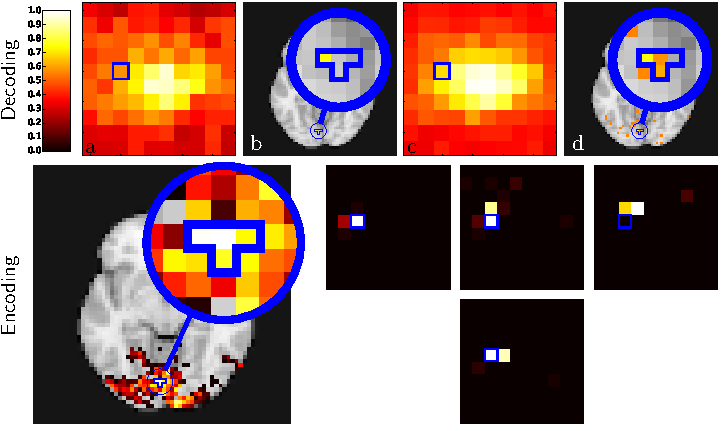
\includegraphics[width=\linewidth]{img/miyawaki/figure}
  \end{center}
  \caption{
      Miyawaki results in both decoding and encoding. Highlighted pixels and
      voxels are the same across methods. Results are consistent as decoding
      and encoding have found a relation between the same pixel and voxels.
      \textbf{Decoding.} Reconstruction accuracy per pixel (\textit{a.} Logistic
      regression, \textit{c.} SVC). Coefficients used to predict the chosen pixel(\textit{b.} Logistic
      regression, \textit{d.} SVC). 
      \textbf{Encoding.} Left: reconstruction accuracy depending on pixel
           position in the stimulus. Right: receptive fields corresponding to
       voxels with highest scores and neighbours.}
\label{fig:miyawaki}
\end{figure}


\section{Resting-state and functional Connectivity analysis}

Even in the absence of external behavioral or clinical variable, studying
the structure of brain signals can reveal interesting information.
Indeed, \cite{biswal1995} have shown that brain activation exhibits
coherent spatial patterns during rest. These correlated voxel activations
form functional networks that are consistent with known task-related networks.

Biomarkers found via predictive modeling on resting-state fMRI would be
particularly useful, as they could be applied to diminished subjects that
cannot execute a specific task. Here we use a dataset containing control
and ADHD (Attention Disorder Hyperactivity Disorder) patients resting
state data (subjects are scanned without giving them any specific task to
capture the cerebral background activity).

Resting state fMRI is unlabeled data in the sens that the brain activity
at a given instant in time cannot be related to an output variable.
In machine learning, this class of problems is known as unsupervised
learning. 
To extract functional networks or regions, we use methods that group together 
similar voxels by comparing their time
series. In neuroimaging, the most popular method is ICA and
is the subject of our first example. We will then show how to obtained 
functionally-homogeneous regions with
clustering methods.

\subsection{Independent Component Analysis (ICA) to extract networks}

\subsubsection{Principle}

ICA is a blind source separation method. Its principle is to separate a
multivariate signal into several components by maximizing their non-Gaussianity.
A typical example is the \emph{cocktail party problem} where ICA is able to separate
voices from several people using signal from microphones located across the room.

ICA is the reference method to extract networks from resting state
fMRI \citep{kiviniemi2003}. Several strategies have been used to syndicate ICA
results across several subjects. \cite{calhoun2001a} propose a dimension
reduction (using PCA) followed by a concatenation of timeseries (used in this
example). \cite{varoquaux2010} use dimension reduction and canonical correlation analysis
to aggregate subject data. Melodic, ICA program from the FSL suite uses a Tensor
ICA approach which is not detailed here.

\subsubsection{Application}

As data preparation steps, we not only center, but also detrend the time
series to avoid capturing linear trends with the ICA. Applying to the
resulting time series the FastICA algorithm with scikit-learn is
straightforward thanks to the transformer concept. The data matrix must
be transposed, as we are using \emph{spatial} ICA, in other words the
direction considered as random is that of the voxels and not the time
points. The maps obtained capture different components of the signal,
including noise components as well as resting-state functional networks.


\begin{lstlisting}
# Here we start with Xs: a list of subject-level data matrices
# First we concatenate them in the time-direction, thus implementing
# a concat-ICA
X = np.vstack(Xs)
from sklearn.decomposition import FastICA
ica = FastICA(n_components=20)
components_masked = ica.fit_transform(data_masked.T).T
\end{lstlisting}

\subsubsection{Results}

On fig. \ref{fig:ica} we compare a simple concat ICA as implemented by
the code above to more sophisticated multi-subject methods, namely CanICA
and MELODIC's concat ICA. We display here only the default mode network
as it is a well-known resting-state network.

\begin{figure}[hbtp]
  \begin{center}
      \begin{subfigure}[b]{.3\linewidth}
        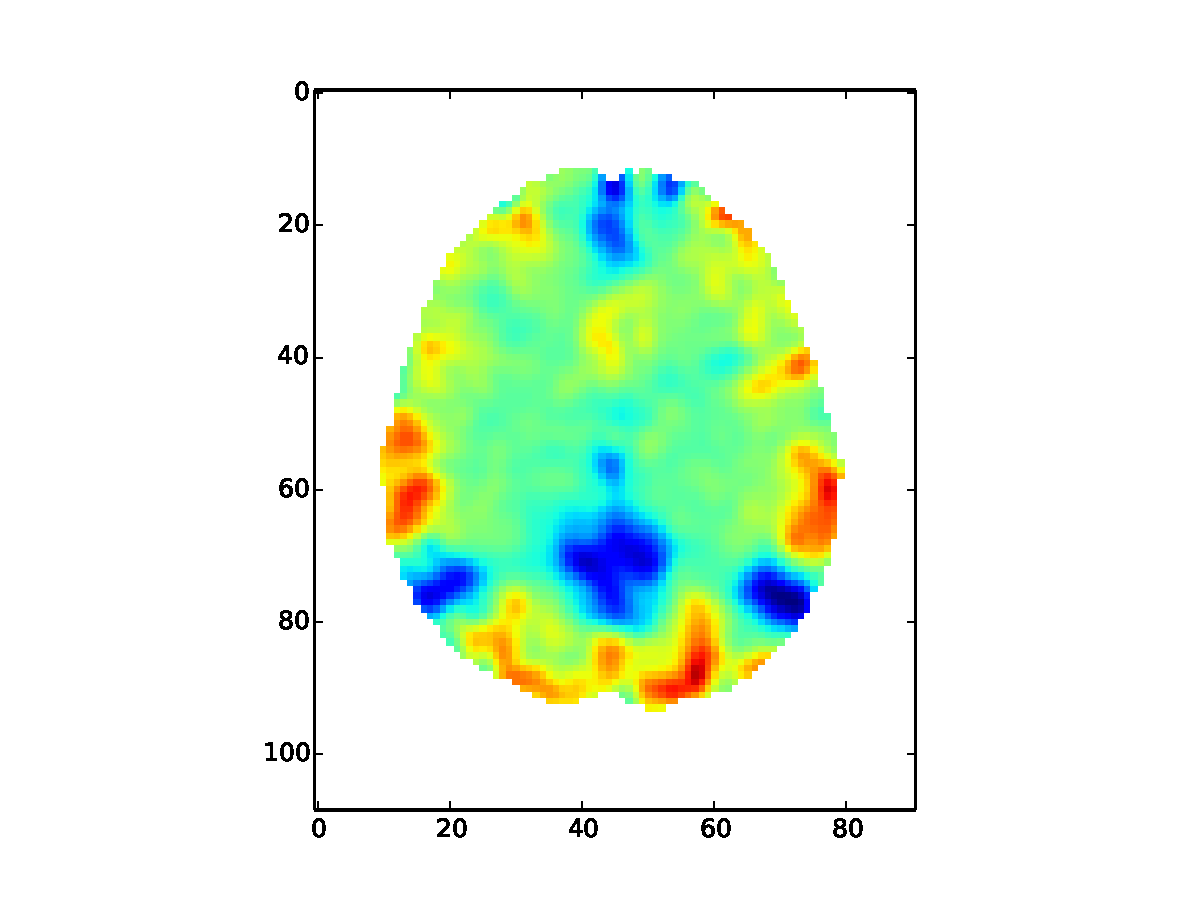
\includegraphics[width=\linewidth]{img/ica/ica}
        \caption{ICA}
      \end{subfigure}
      \begin{subfigure}[b]{.3\linewidth}
        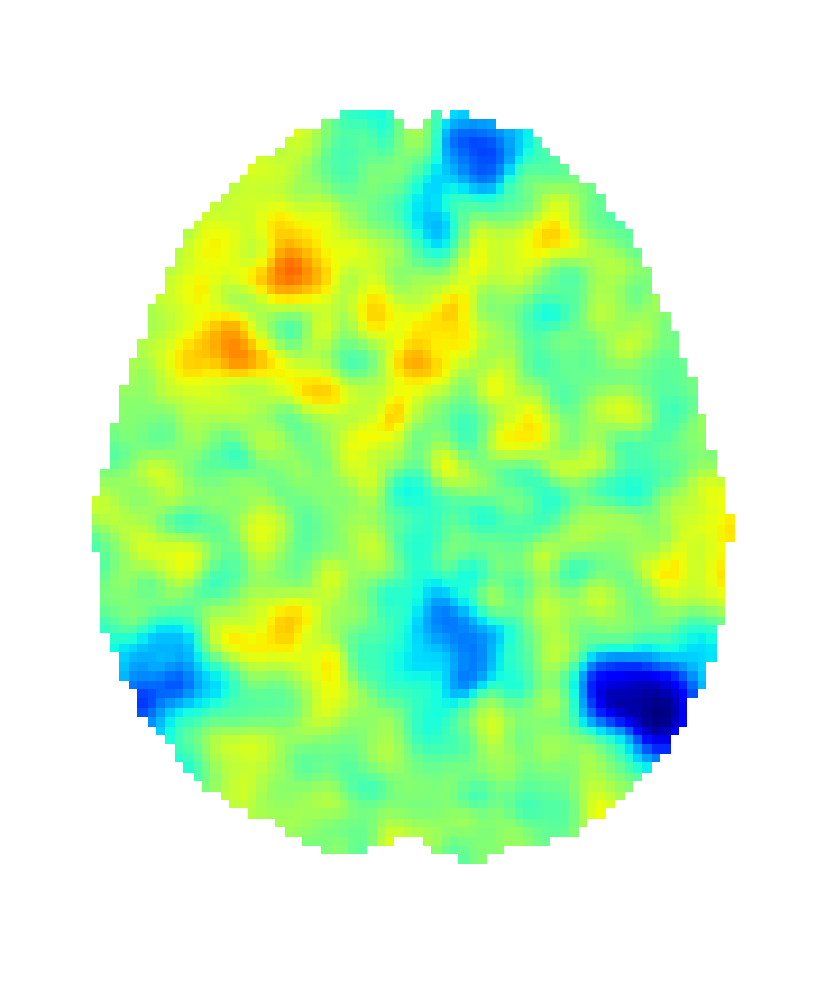
\includegraphics[width=\linewidth]{img/ica/canica}
        \caption{CanICA}
      \end{subfigure}
      \begin{subfigure}[b]{.3\linewidth}
        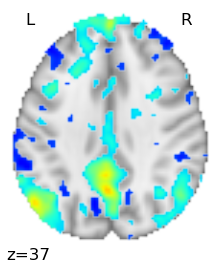
\includegraphics[width=\linewidth]{img/ica/melodic}
        \caption{melodic}
      \end{subfigure}
  \end{center}
  \caption{Default mode network extracted using different approaches:
\emph{left}: the simple Concat-ICA approach demoed in this article;
\emph{middle}: CanICA, as implemented in nilearn; \emph{right}: Melodic's
concac-ICA.}
  \label{fig:ica}
\end{figure}

\subsection{Learning functionally-homogeneous regions with clustering}
\label{clustering}

From a machine learning perspective, a clustering method aggregates 
samples into groups (called clusters) to maximize a measure of similarity in
the clusters. If we consider voxels of a functional brain image, this 
measure can capture functional similarity, thus the clusters of voxels
form functionally-homogeneous regions \citep{thirion2006}.

\subsubsection{Imposing spatial structure}

\subsubsection{Approaches}

Several clustering approaches exists, each one having its own pros and
cons. Most require setting the number of clusters extracted. This choice
depends on the application: a large number of cluster will give a more
fine-grained description of the data, with a higher fidelity to the
original signal, but also a higher model complexity. Some clustering
approaches can make use of spatial information and yield
spatially-contiguous clusters, \emph{i.e.} parcels. Here we will describe
two clustering approaches that are simple and fast.

\paragraph{Ward clustering} uses a bottom-up hierarchical approach:
progressively agglomerating voxels together into clusters. In
scikit-learn, structural information can be specified via a connectivity
graph given to the Ward clustering estimator. This graph is used to allow
only merges between neighboring voxels, thus readily producing contiguous
parcels. We will rely on the {\tt
sklearn.feature\_extraction.image.grid\_to\_graph} function to
construct such a graph using the neighbor structure of an image grid,
with optionally a brain mask.

\paragraph{K-means} is a more top-down approach, seeking cluster centers
to evenly explain the variance of the data. Each voxels are then assigned
to the nearest center, thus forming clusters. As imposing a spatial model
in K-means is not easy, it is often advisable to spatially-smooth the
data.

To apply the clustering algorithms, we run the common data preparation
steps and produce a data matrix. As both Ward clustering and K-means rely
on second-order statistics, we can speed up the algorithms by reducing
the dimensionality while preserving these second-order statistics with a
PCA. Note that clustering algorithms group samples and that here we want
to group voxels. So if the data matrix is, as previously a (time points
$\times$ voxels) matrix, we need to transpose it before running the
scikit-learn clustering estimators. Scikit-learn provides a
\texttt{WardAgglomeration} object to do this \emph{feature agglomeration}
with Ward clustering \cite{michel2012supervisedclustering}, but this is
not the case when using K-Means.

\begin{lstlisting}
connectivity = grid_to_graph(n_x=mask.shape[0], n_y=mask.shape[1],
                             n_z=mask.shape[2], mask=mask)
ward = WardAgglomeration(n_clusters=1000, connectivity=connectivity)
ward.fit(X)
\end{lstlisting}

\subsection{Results}

Clustering results are shown in figure~\ref{fig:clustering}. Cluster colors are
random. These clustering does not contain neuroscientifc information. However,
as clustering group similar voxels together, it can be used as a compression
method more sophisticated than the simple downsampling.
% Discuss the 'compression intuition'

\begin{figure}[hbtp]
  \begin{center}
      \begin{subfigure}[b]{.23\linewidth}
          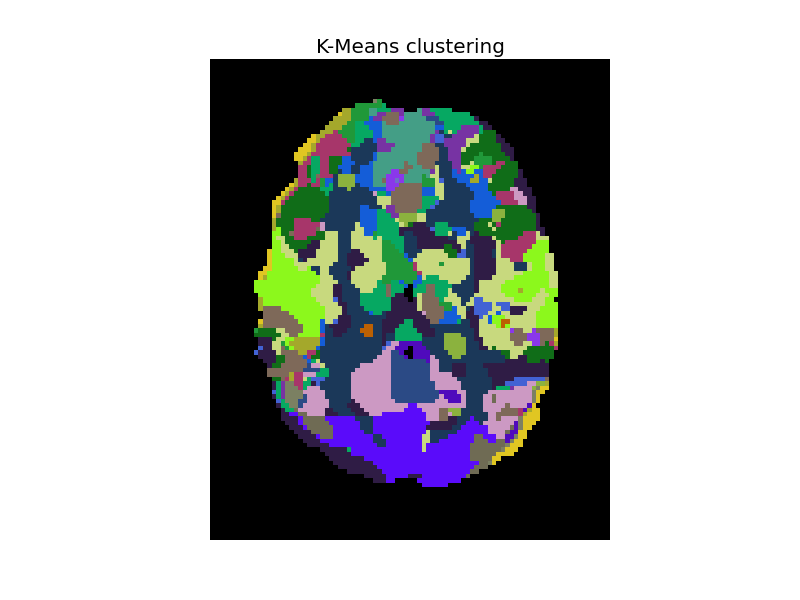
\includegraphics[width=\linewidth]{img/clustering/kmeans}
        \caption{K-Means}
      \end{subfigure}
      \begin{subfigure}[b]{.23\linewidth}
        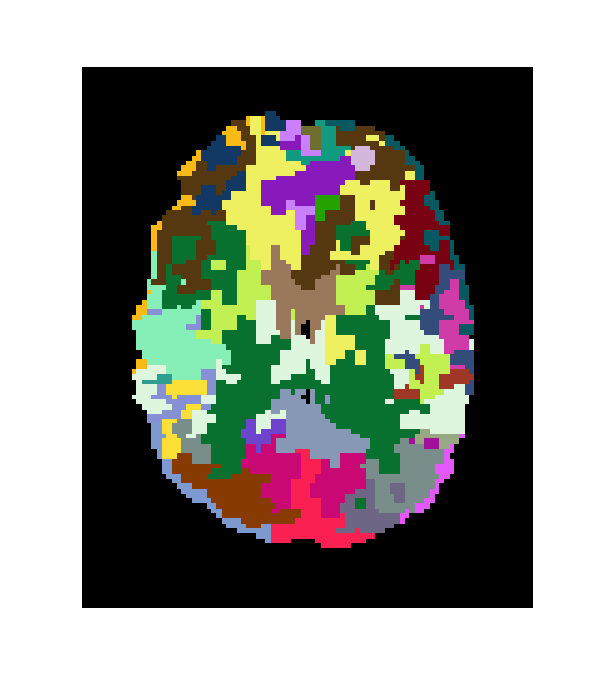
\includegraphics[width=\linewidth]{img/clustering/ward}
        \caption{Ward's clustering}
      \end{subfigure}
      \begin{subfigure}[b]{.23\linewidth}
        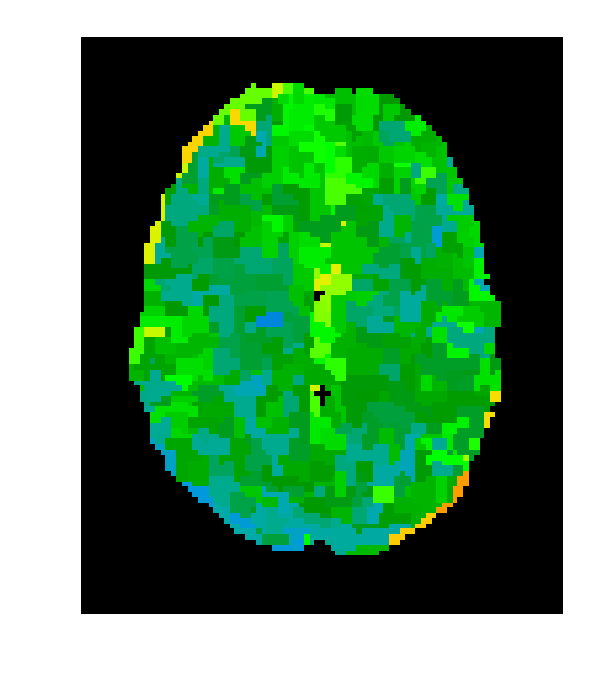
\includegraphics[width=\linewidth]{img/clustering/ward_compressed}
        \caption{Ward's compression}
      \end{subfigure}
      \begin{subfigure}[b]{.23\linewidth}
        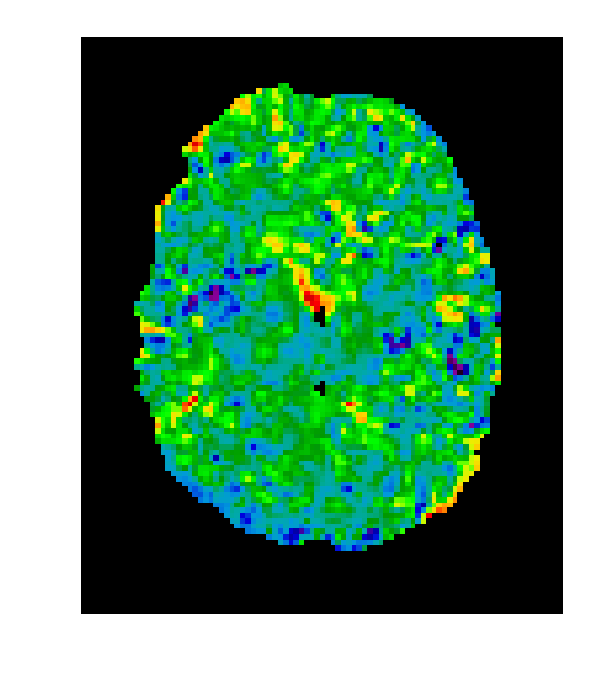
\includegraphics[width=\linewidth]{img/clustering/original}
        \caption{Original signal}
      \end{subfigure}
  \end{center}
  \caption{Brain decomposition using Ward's clustering and Kmeans. (c) shows how the original
  signal (d) is compressed using the Ward's clustering decomposition (b).}
  \label{fig:clustering}
\end{figure}

\section{Conclusion}

These use cases show that neuroscientific problems can be easily handled thanks
to scikit-learn python library. Difficulties lie in applying proper preprocessing of
the data, chosing the right model depending on the problem and interpreting
these results. An attempt to
address the first problem has been made in the nilearn Python library which
provides convience tools to load neuroscientific data. However, the other
problems require skill and experience.

% XXX: note that the techniques described in this paper only scratch the
% surface of the applications of statistical learning in neuroimaging. 

\section*{Disclosure/Conflict-of-Interest Statement}
%All relationships financial, commercial or otherwise that might be perceived
%by the academic community as representing a potential conflict of interest
%must be described. If no such relationship exists, authors will be asked to
%declare that the research was conducted in the absence of any commercial or
%financial relationships that could be construed as a potential conflict of
%interest.
The authors declare that the research was conducted in the absence of any
commercial or financial relationships that could be construed as a potential
conflict of interest.

\paragraph{Funding\textcolon} We acknowledge funding from the NiConnect project.

\bibliographystyle{frontiersinSCNS} % for Science articles
\bibliography{biblio}

\end{document}
